\section{General sewer construction}\label{se:sewer_construction}
This section will elaborate on the general contruction of sewers. Furthermore a brief explanation, of the flow into the sewer to the output from the wastewater treatment plant (WWTP), is given.

%This section will elaborate on the general construction of a sewer. Furthermore a general explanation of the transport of wastewater undergoes from households/industry to it is treated at the plant will be elaborated.    

Generally sewer construction can be put into two categories which are gravity and pressure sewers. Gravity sewers utilize the topographic advantages of the area in which they are constructed. But in places where the level of the surface area does not accommodate a slope of the sewer pipe, such that wastewater flow in the desired direction, wells with pumps are used to transport the wastewater to an elevated level. An illustration of gravity and pressure sewer lines can be seen in figure \ref{fig:Sewer_drawing}. 

\begin{figure}[H]
\centering
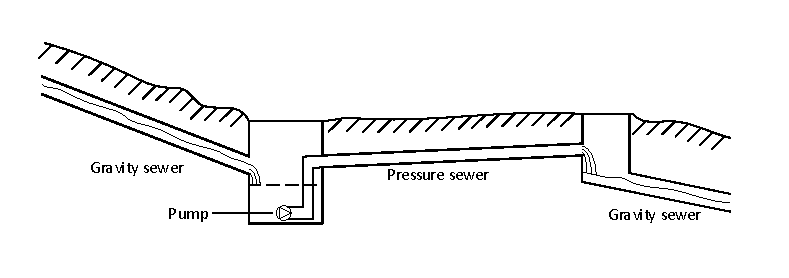
\includegraphics[width=1\textwidth]{report/introduction/pictures/Sewer_drawing.pdf}
\caption{Illustration of flow in gravity and pressured sewer lines.}
\label{fig:Sewer_drawing}
\end{figure}

Design of sewer systems involves careful considerations, such that as much of the network utilize gravity for transport of wastewater, to minimize the energy consumption. Therefore the WWTP is typically located in a low topographic area near a river, fjord or the sea. Other design parameters involves dimensioning of the pipes to avoid overflow and to compensate for groundwater ingress into the sewer lines.
%the depth in which they are placed in the ground. 
Also the depth should be sufficiently, such that subzero temperatures does not prevent the flow in the sewers at any time. Furthermore the slope of the pipes must be chosen such that sufficient flow is obtained and clogging is avoided. Different materials used to create the pipes gives different amount of friction e.g. a concrete surface will be more rough than polyethylene and thereby have a higher friction. This means that a larger slope of a concrete pipe is needed to avoid clogging. Typically gravity sewer pipes is made of concrete and pressure sewer pipes of polyethylene.

In figure \ref{fig:sewer_overview_of_the_different_parts} a block diagram of the flow of wastewater is seen.
\begin{figure}[H]
\centering
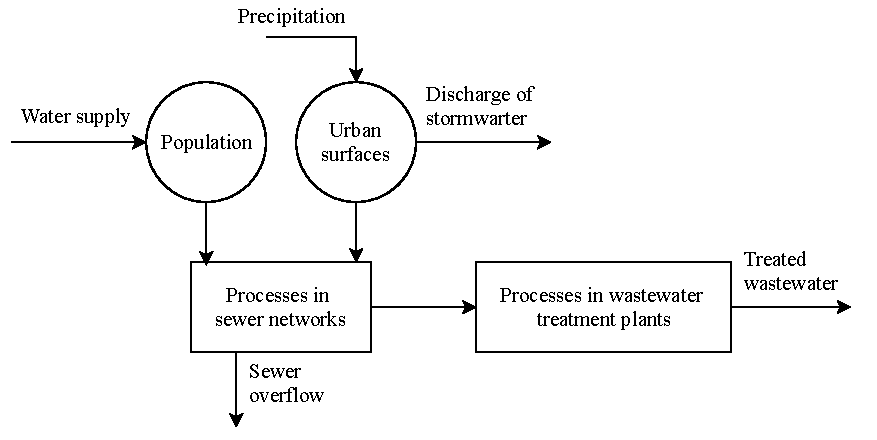
\includegraphics[width=0.9\textwidth]{report/introduction/pictures/sewer_process2.pdf}
\caption{General overview of the flow of wastewater from users and surface runoff to the treated water is released into receiving waters. Arbejdsblad billede, inspiration er taget fra hvitved. Fjern sludge handling of floc separation og forklar det nede ved afsnittet.}
\label{fig:sewer_overview_of_the_different_parts}
\end{figure}

Starting at the left side in the figure, precipitation from urban surfaces and roads are let into the sewer by inlets placed at the gutter. In recent times separate sewer systems for surface runoff are constructed, which are also called storm water sewers. The water in these sewers are typically led in to storm water basins, rivers or the sea. In areas with older sewer constructions storm water is let into sewers where it is mixed with wastewater. The wastewater comes from households or industry disposing of substances of varying consistency. Heavy precipitation can cause the sewers to be filled, and to avoid overflow, into household or on roads, the wastewater is let into rivers or the sea during such events. 
The reason for designing storm water sewers is partly to avoid letting untreated sewage into the nature, but also to better be able to control the cleansing process at the WWTP. %It is desirable to have a steady flow of wastewater with a steady level of chemical concentration flowing into the WWTP.
When wastewater is received at the treatment plant it undergoes several processes to separate the unwanted substances from the received wastewater. Afterward the cleansed water is released into nearby rivers or the sea.
Due to the the sizes of sewer networks, which can have inlets several kilometers from the WWTP, reactions also occurs in the sewer pipes.
The chemical and microbial reactions happening in the sewer lines is discussed in subsection \ref{subse:chemical_reactions_in_a_sewer}. The processes which the wastewater undergoes at the treatment plant is discussed in subsection \ref{subse:Wastewater treatment plant}.  

%From the left in the figure the precipitation over urban surfaces are collected in the sewer. If the precipitation are to extreme for the sewer to handle it will be discharged in a storm water sewer, which will lead the water into small rivers or be collected in tanks \fxnote{Skriv hvad det bliver brugt til}. Furthermore from the left the water supplies goes into the consumers of the water, such as the industry or households. These will produce wastewater that is lead into the sewers. Within the sewers chemical and microbial reactions occurs, which will be explained in subsection \ref{subse:chemical_reactions_in_a_sewer}. If the sewer is overfilled the wastewater is lead into rivers and fields to prevent flooding in households, industry and urban surfaces. The sewer leads the wastewater to the wastewater treatment plant, where the wastewater will be filtered before sending it back into the environment, which will be explained in greater detail in subsection \ref{subse:Wastewater treatment plant}.
%The water treatment plant are constructed near rivers or a fjord which is often at a lower geographical location, thereby enabling the force of gravity to transport the wastewater in a sewer. If the industry or the households are at a lower geographical location than the water treatment plant, then pumps are used to transport the wastewater as illustrated in figure \ref{fig:Sewer_drawing}.
% \begin{figure}[H]
% \centering
% 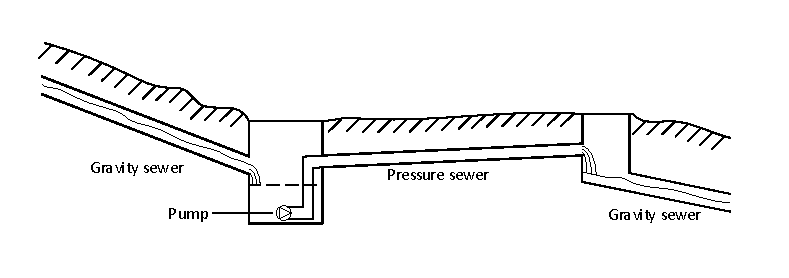
\includegraphics[width=1\textwidth]{report/introduction/pictures/Sewer_drawing.pdf}
% \caption{Illustrate different methods for transportation of wastewater.}
% \label{fig:Sewer_drawing}
% \end{figure}
%These pipes are often constructed in concrete or polyethylene. Where concrete pipes are used for gravity sewers and polyethylene are used in a pressure sewer due to a lower roughness height which means less friction from the surface of the pipe. 